\documentclass{beamer}

\mode<presentation> {
  \usetheme{Frankfurt}
  \setbeamercovered{transparent}
}

\usepackage[utf8]{inputenc}
\usepackage{graphicx}
\usepackage{subfig}
\usepackage[czech]{babel}

\title{Mobilní aplikace Florbalový trenér pro iOS}
\author{Jakub Olejník \\
\emph{vedoucí} Ing. Josef Gattermayer}
\institute[ČVUT FIT]{Katedra softwarového inženýrství\\
Fakulta informačních technologií\\
ČVUT v Praze}
\date{19.~6.~2014}

\begin{document}

\begin{frame}
  \titlepage
\end{frame}

\section{Zadání práce}

\begin{frame}
  \frametitle{Obsah}
  \tableofcontents[currentsection]
\end{frame}

\subsection{Zadání}
\begin{frame}
\frametitle{Zadání}

\begin{itemize}
  \item Analyzujte aplikace zabývající se přípravou florbalových tréninků.
  \item Analyzujte požadavky vybraných trenérů na takovou aplikaci.
  \item Na základě analýzy připravte UML modely.
  \item Vytvořte wireframy uživatelského rozhraní.
  \item Připravte specifikaci, podle které navrhněte prototyp mobilní aplikace.
  \item Funkční prototyp otestujte pomocí akceptačních testů.
\end{itemize}

\end{frame}


\subsection{Motivace}
\begin{frame}
\frametitle{Motivace}

\begin{itemize}
  \item Aplikace zaměřená na florbal neexistuje.
  \item Aplikace pro jiné sporty nepodporují florbalovou notaci.
  \item Odpadají nevýhody využití klasické kreslicí tabule.
\end{itemize}

\end{frame}

\section{Analýza existujících řešení}

\begin{frame}
  \frametitle{Obsah}
  \tableofcontents[currentsection]
\end{frame}

\subsection{CoachNote Hockey And Ringette}

\begin{frame}
\frametitle{CoachNote}

  \begin{figure}[H]
    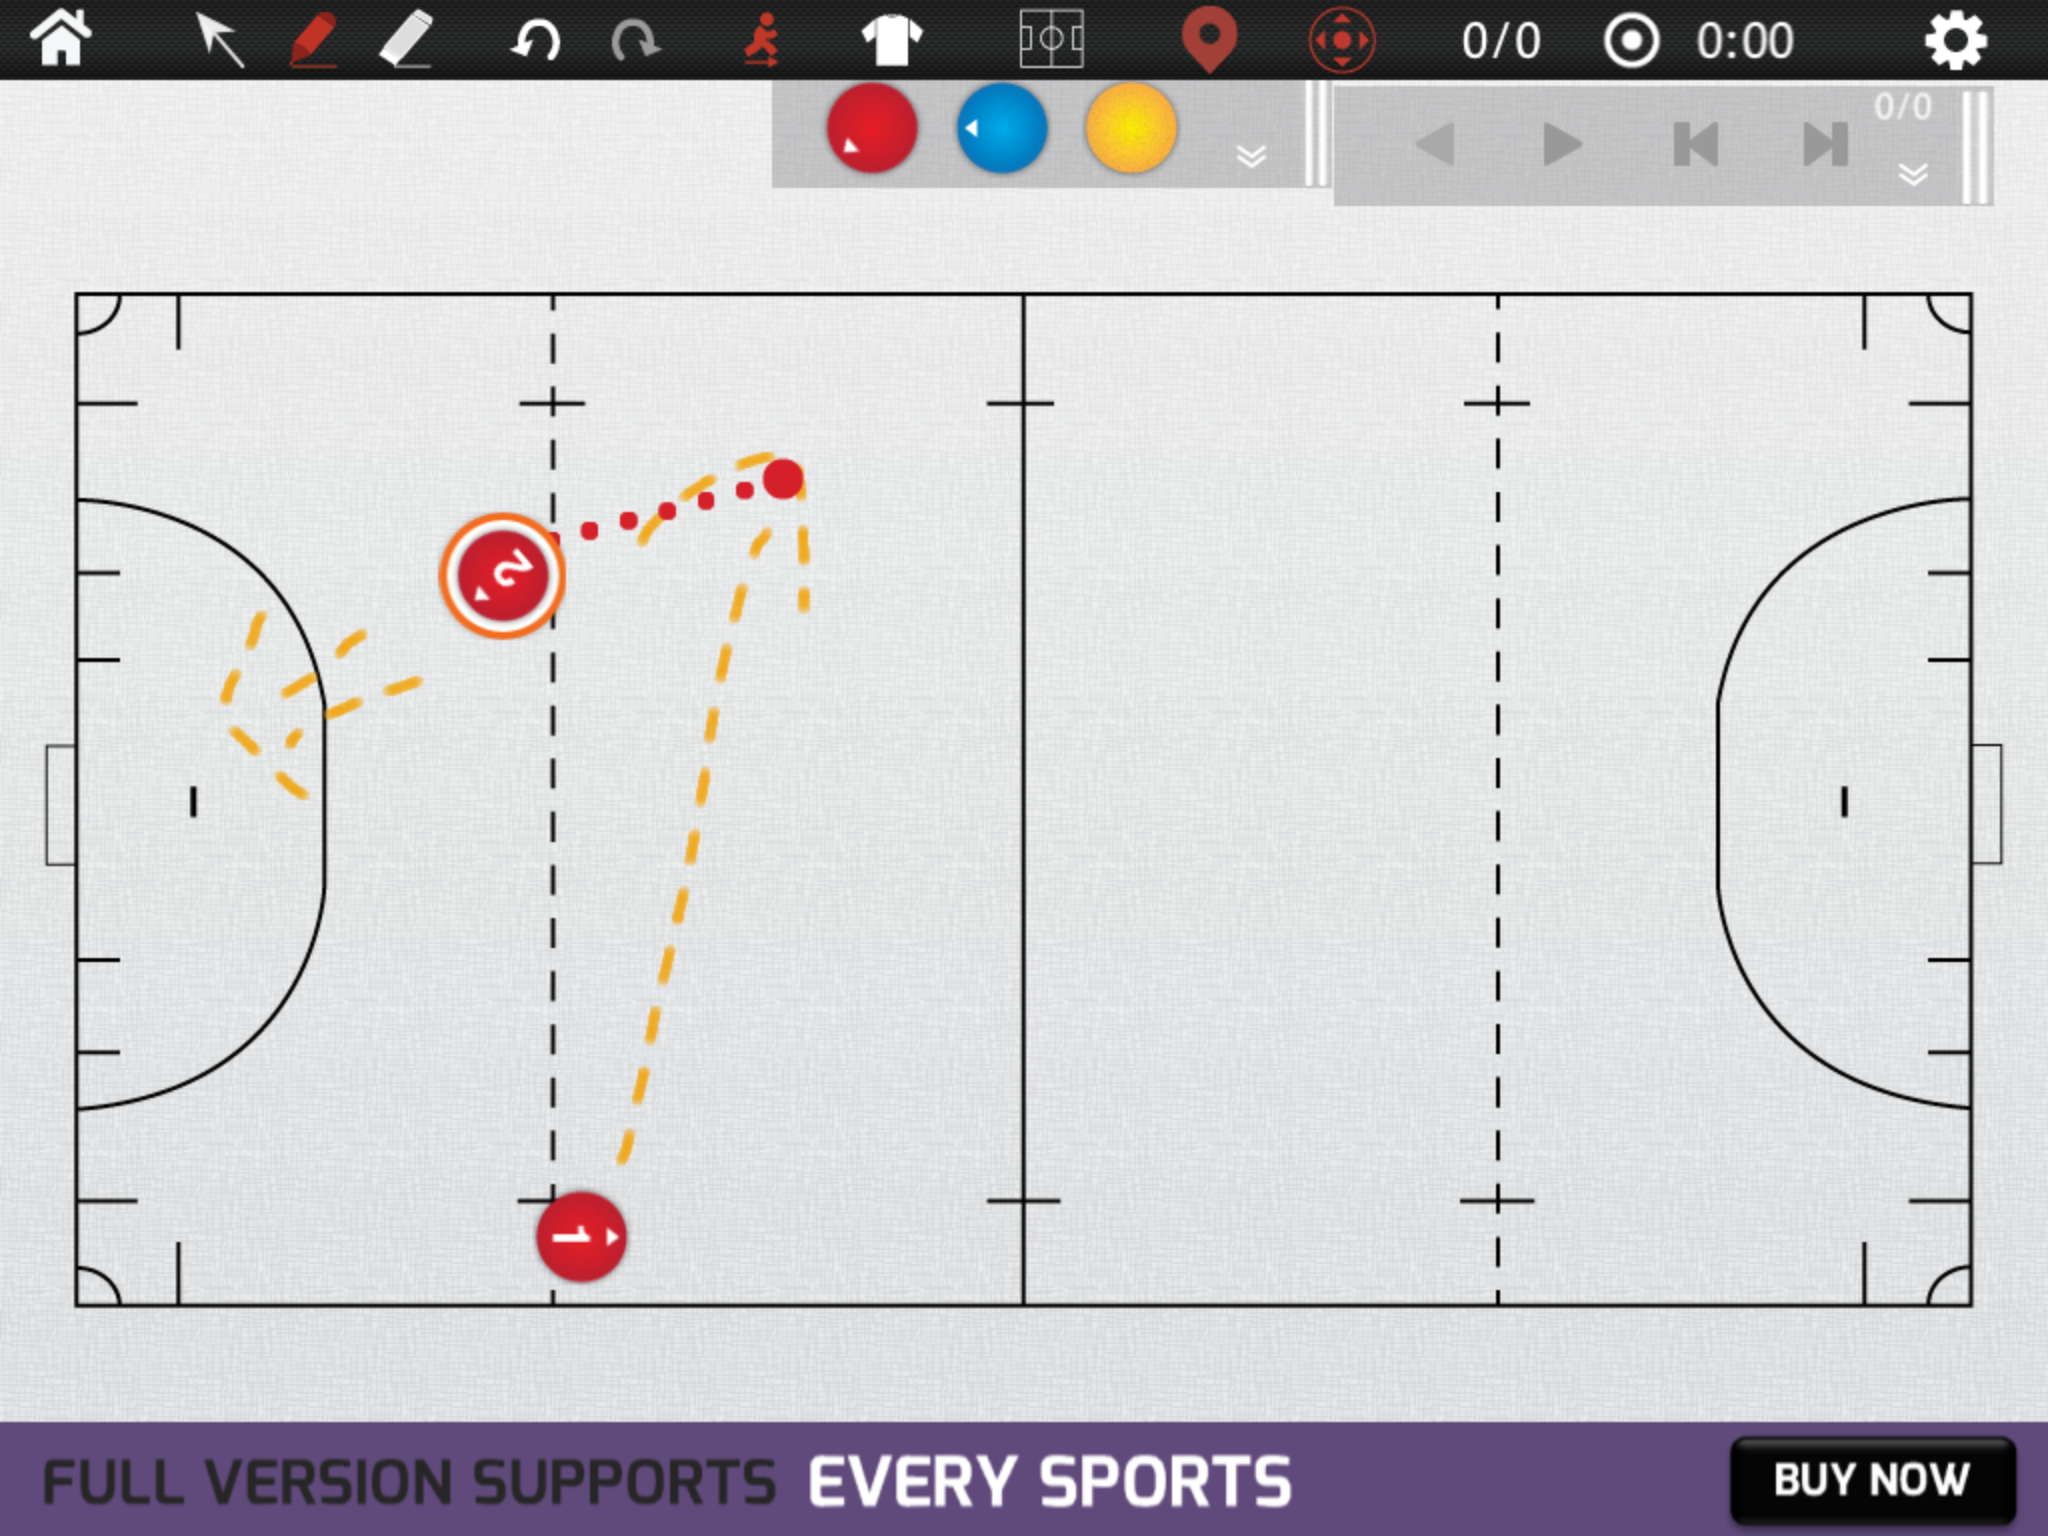
\includegraphics[width=.8\textwidth]{img/IMG_0011}
    \label{pic:coachnote}
  \end{figure}

\end{frame}

\subsection{IceHockey Board Free}
\begin{frame}
\frametitle{IceHockey Board}

  \begin{figure}[H]
    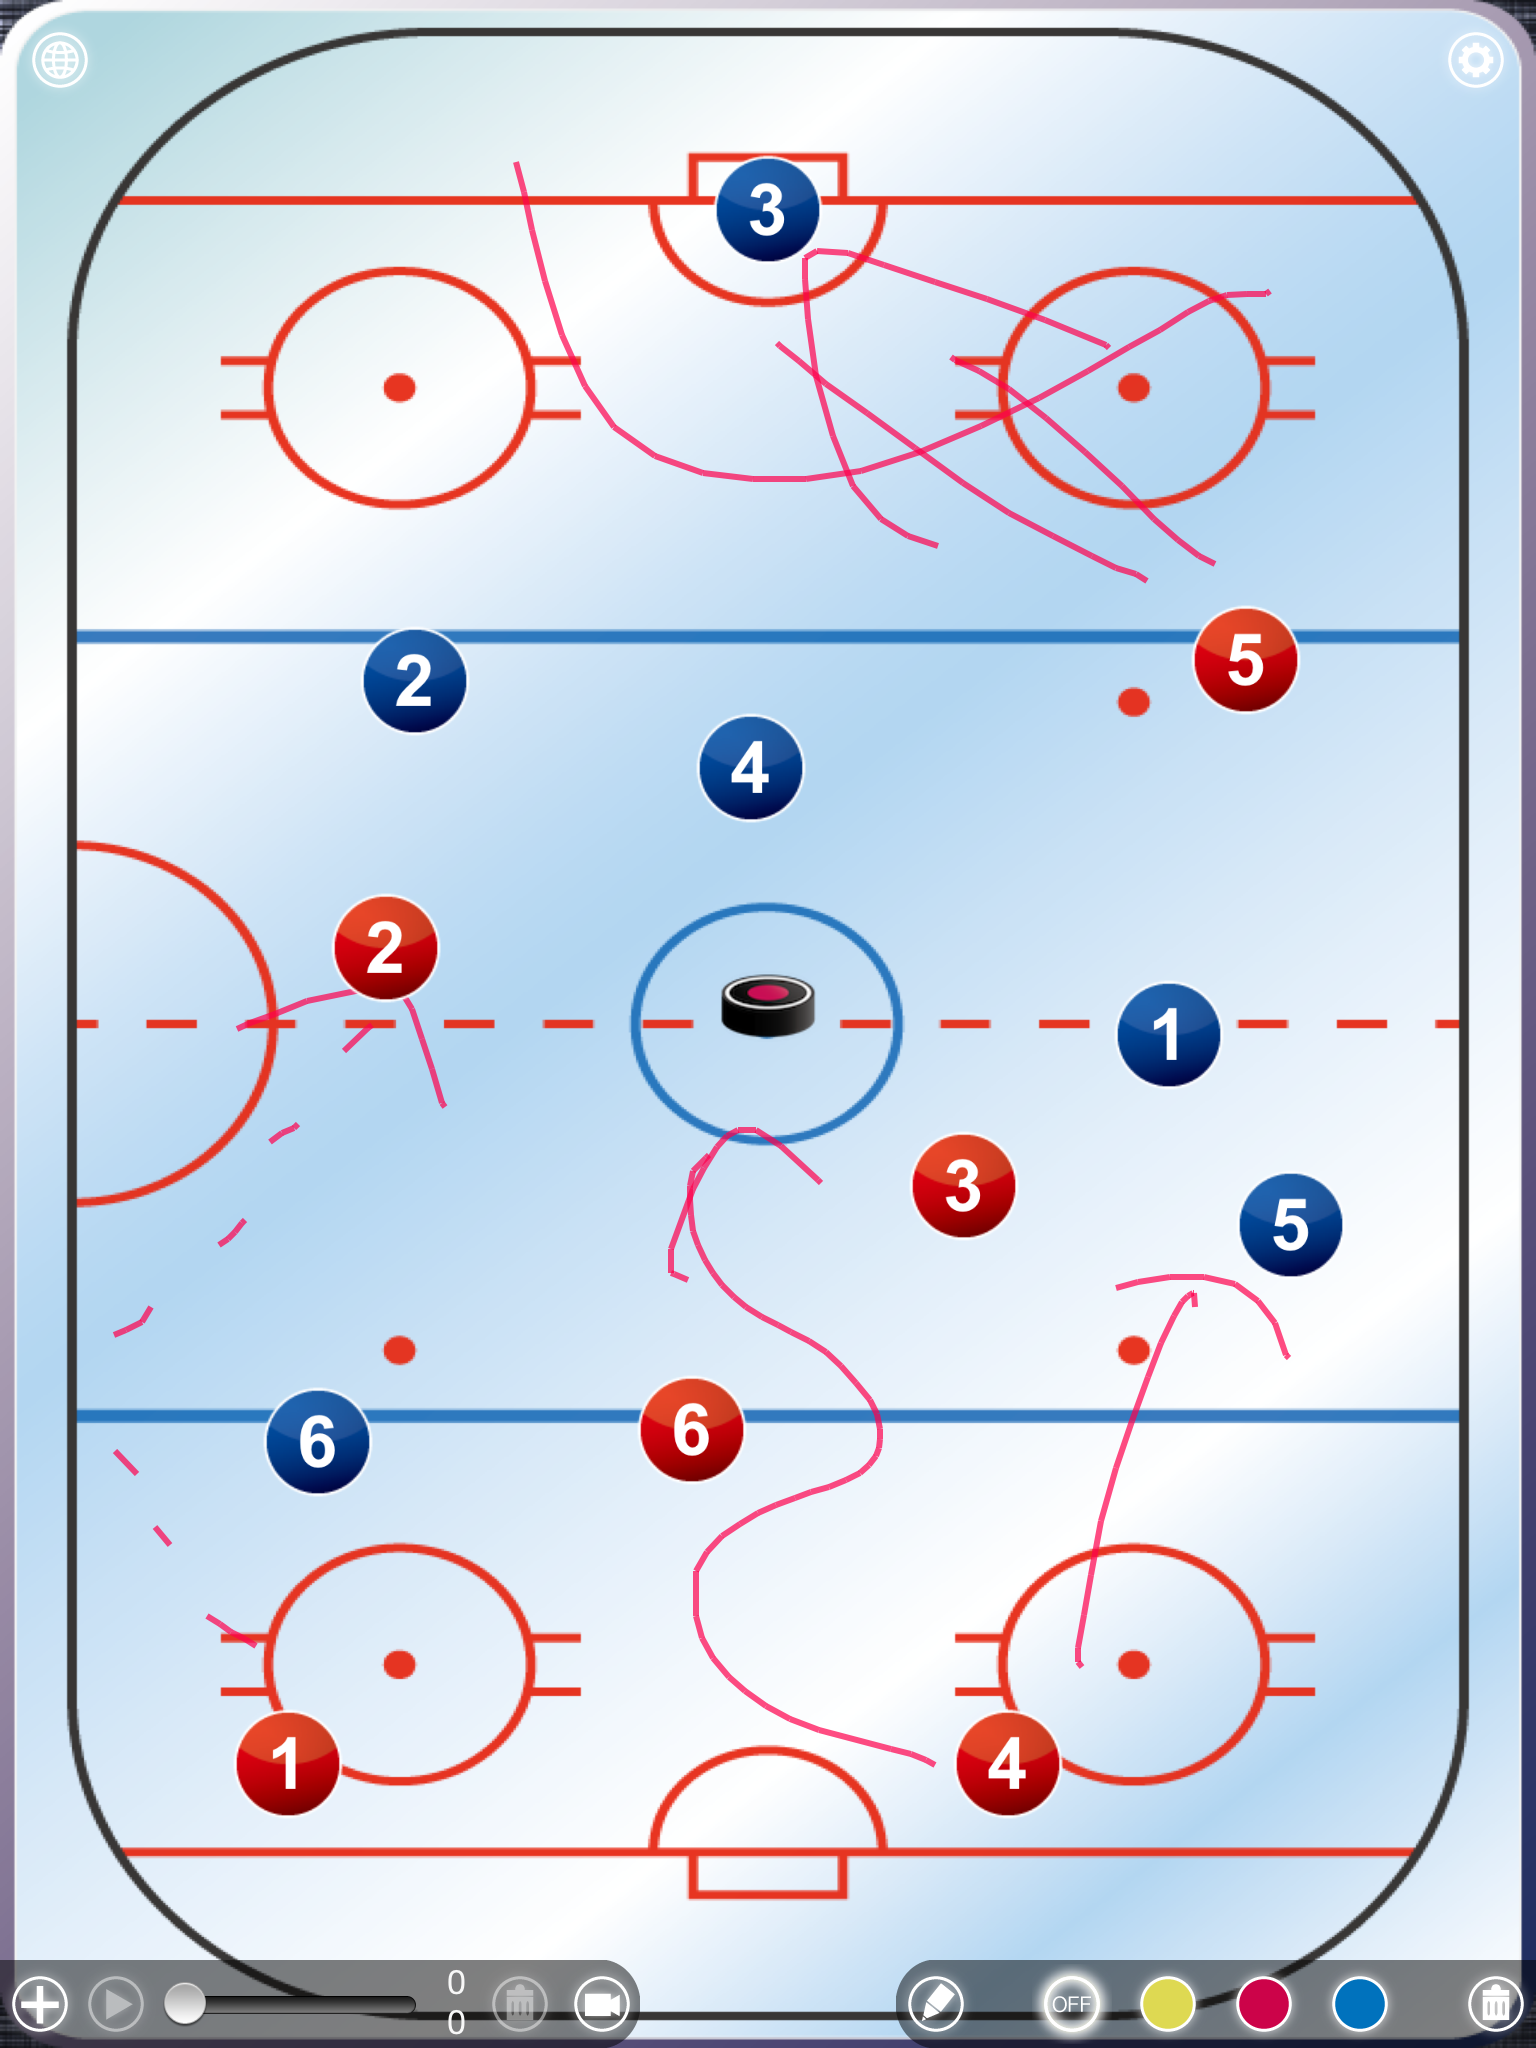
\includegraphics[height=.8\textheight]{img/IMG_0018}
    \label{pic:icehockeyboardfree}
  \end{figure}

\end{frame}

\subsection{My Field Hockey Coach Free}
\begin{frame}
\frametitle{My Field Hockey Coach}
  \begin{figure}[H]
    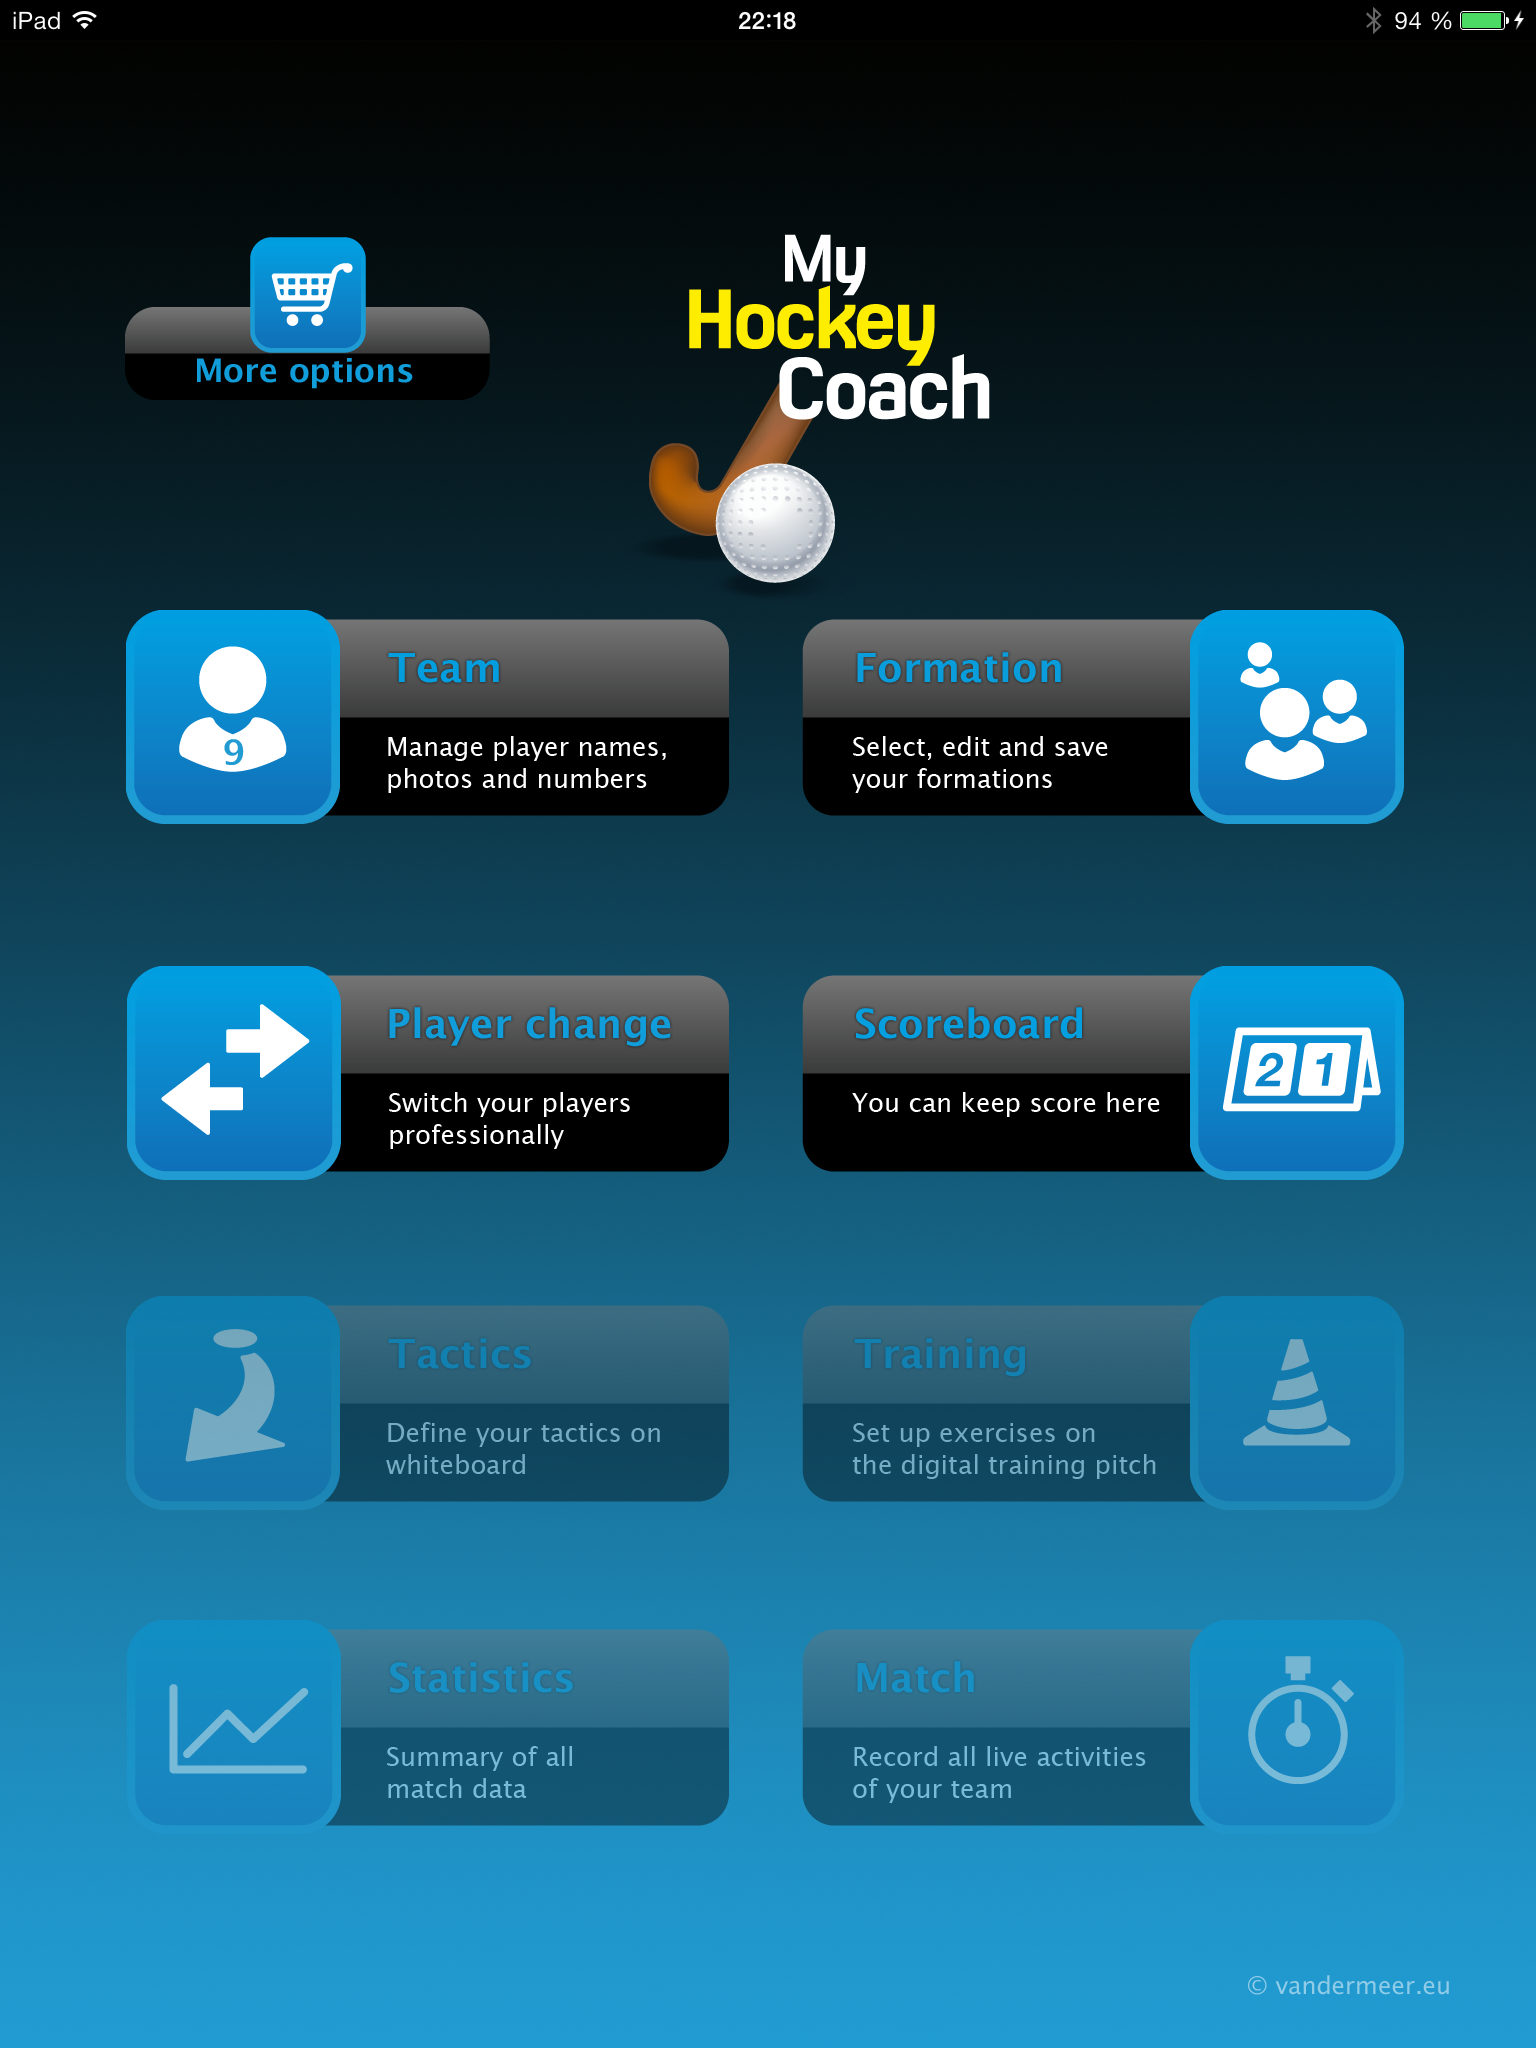
\includegraphics[height=.8\textheight]{img/IMG_0019}
    \label{pic:myfieldhockeycoachfree}
  \end{figure}
\end{frame}

\subsection{Exercise drawer}
\begin{frame}
\frametitle{Exercise drawer}
  \begin{figure}[H]
    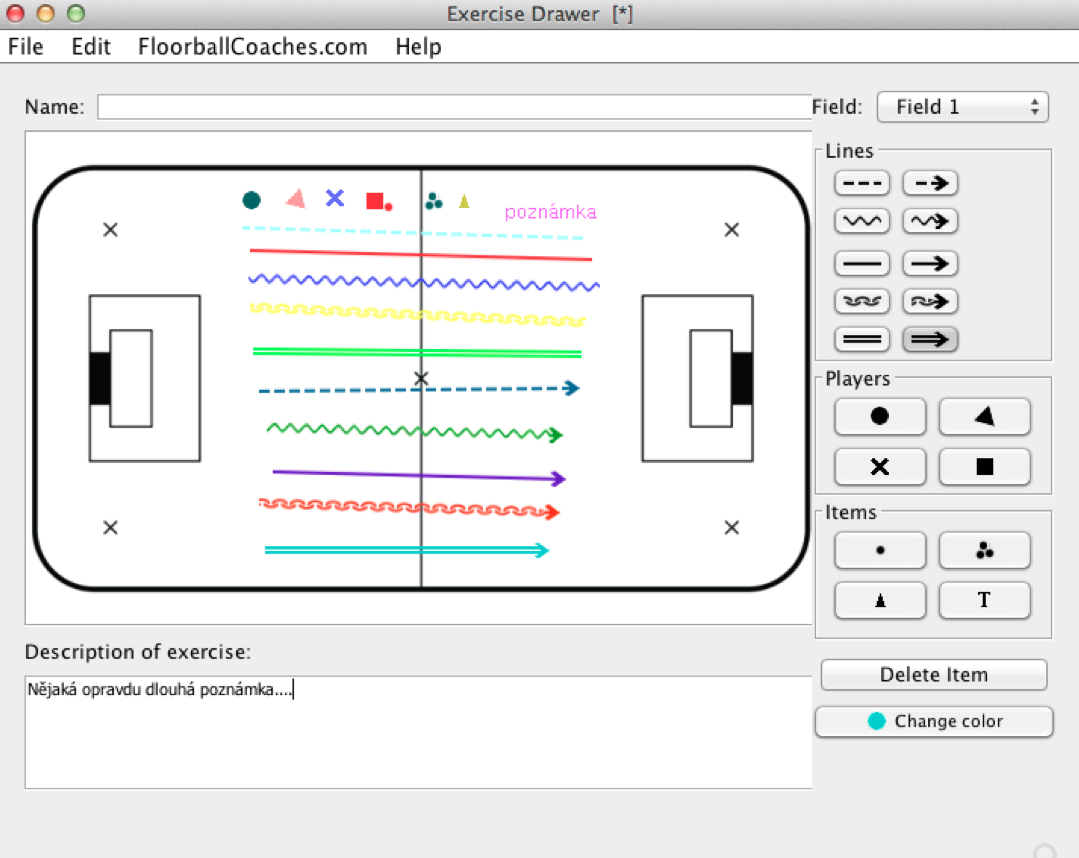
\includegraphics[height=.8\textheight]{img/exercise_drawer}
    \label{pic:exercisedrawer}
  \end{figure}
\end{frame}

\section{Analýza požadavků}

\begin{frame}
  \frametitle{Analýza požadavků}

  Co bylo úkolem analýzy požadavků?

  \begin{itemize}
      \item Zjistit, jaké věkové kategorie budoucí trenéři trénují.
      \item Zjistit, jak často trenéři svěřencům cvičení kreslí.
      \item Zjistit, zda již některý z trenérů využil podobnou aplikaci.
      \item Zjistit, co trenéři od takové aplikace očekávají.
  \end{itemize}
\end{frame}

\section{Návrh aplikace}

\subsection{Navržená funkcionalita}

\begin{frame}
  \frametitle{Navržená funkcionalita}

  \begin{itemize}
    \item volné kreslení na hřiště
    \item předpřipravené nástroje
    \item textové poznámky
    \item perzistentní ukládání cvičení
    \item seskupování cvičení do tréninků
  \end{itemize}
\end{frame}


\subsection{Návrh uživatelského rozhraní}

\begin{frame}
  \frametitle{Návrh uživatelského rozhraní}

  \begin{figure}[H]

    \centering
    \subfloat{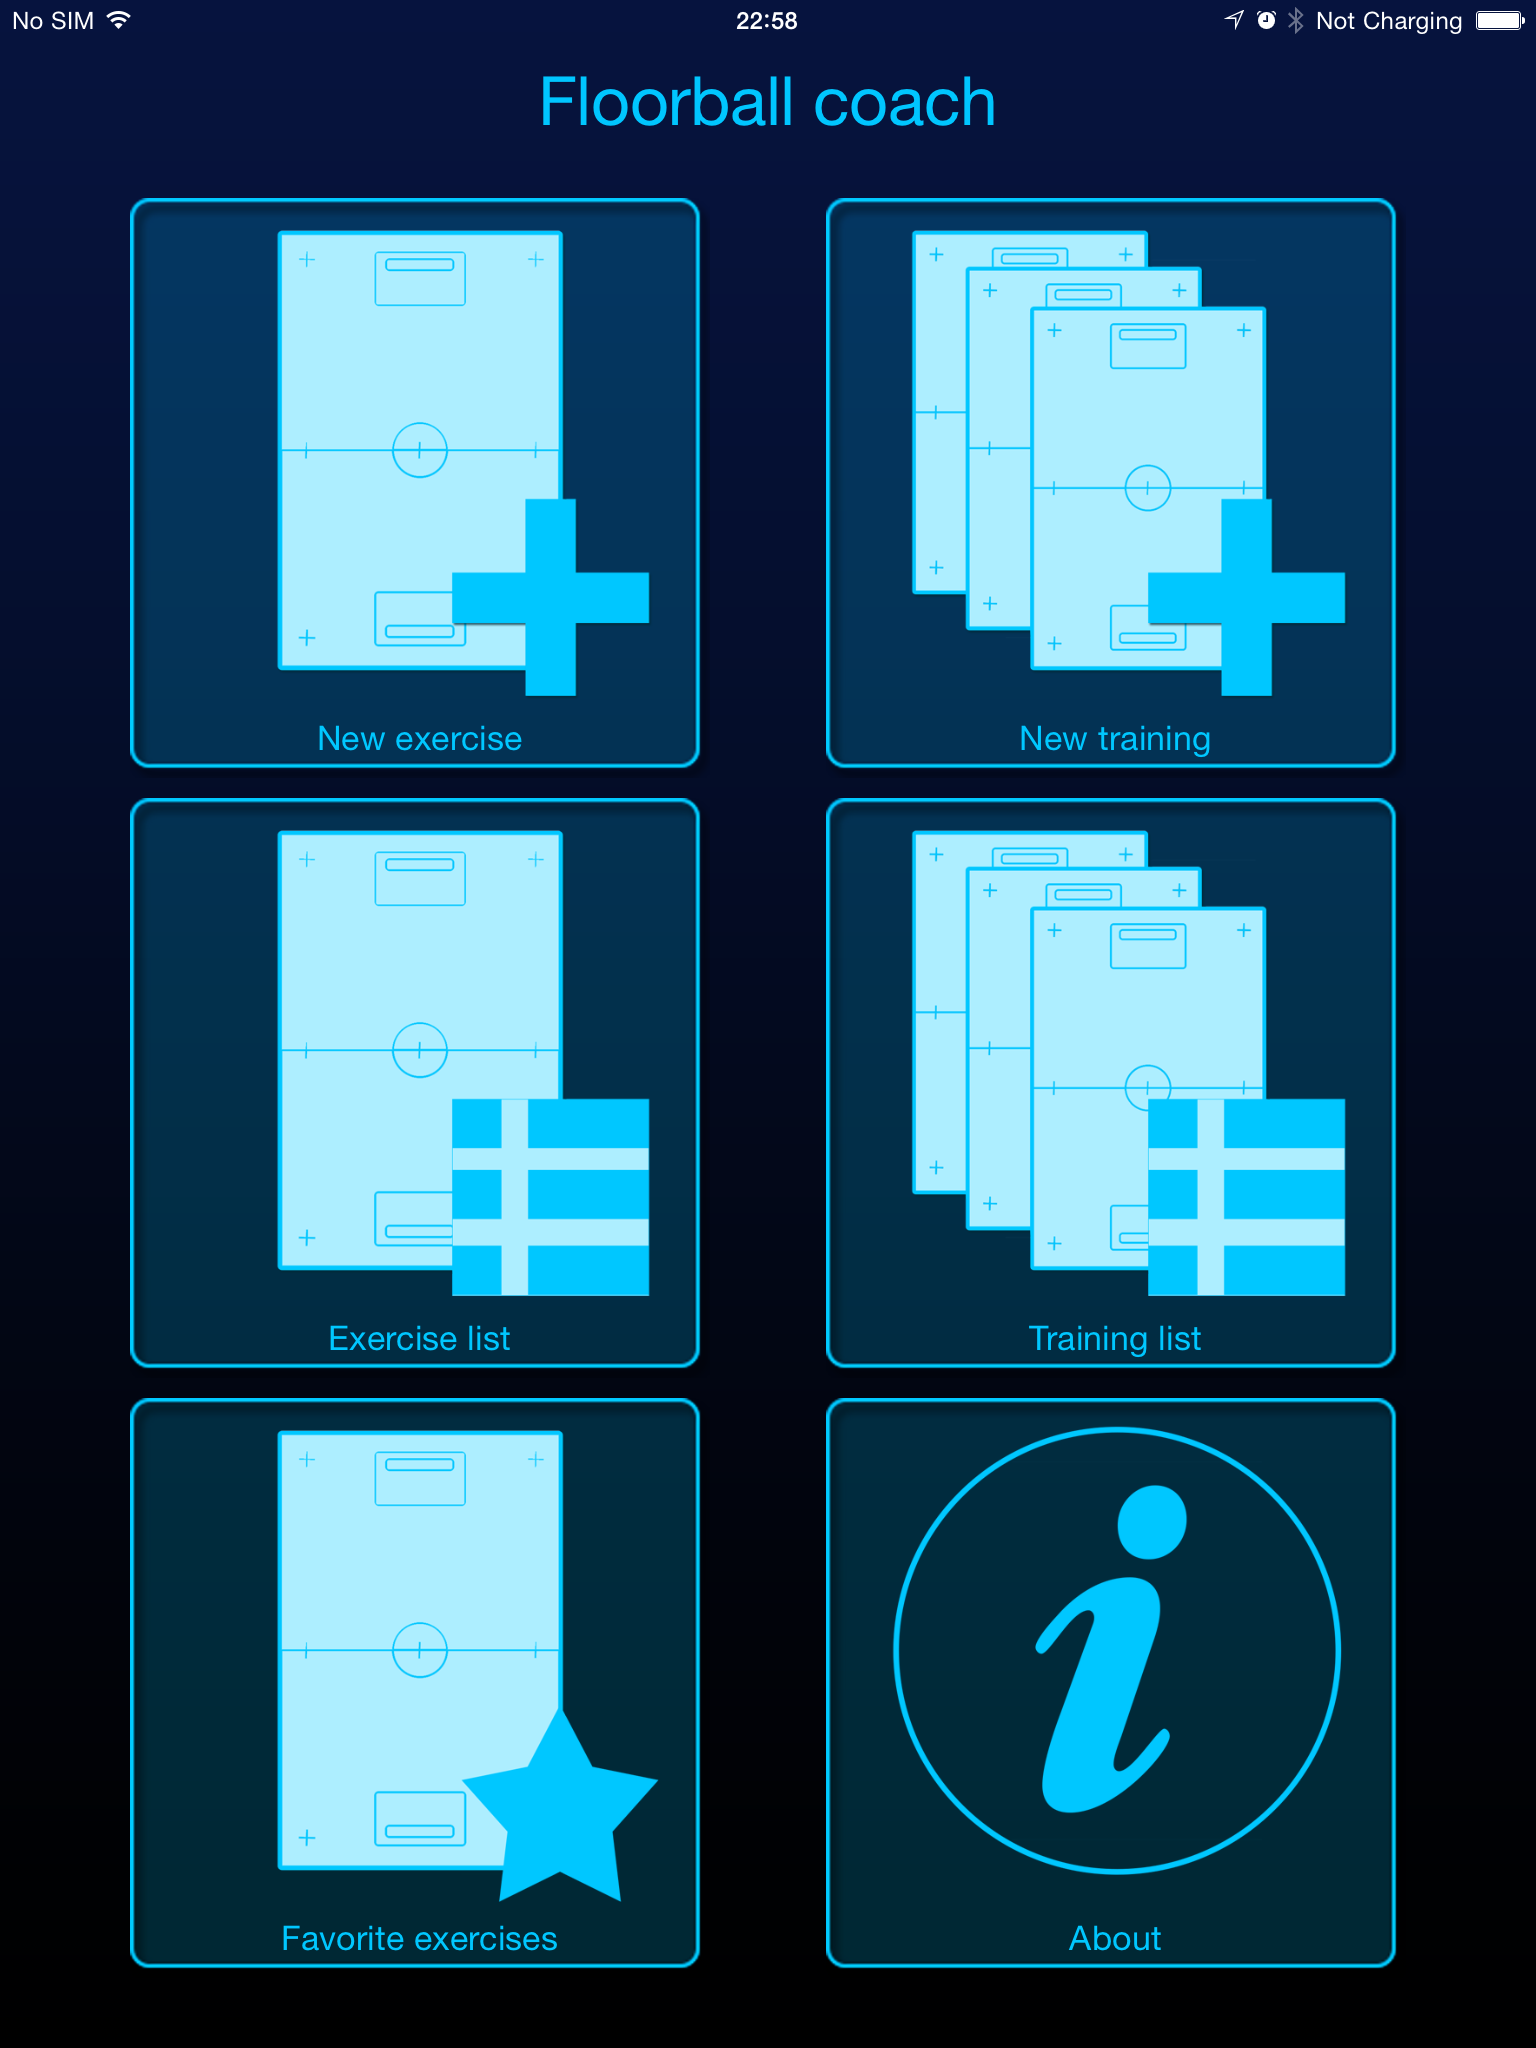
\includegraphics[width=0.4\textwidth]{img/IMG_0277}}
    \hfil
    \subfloat{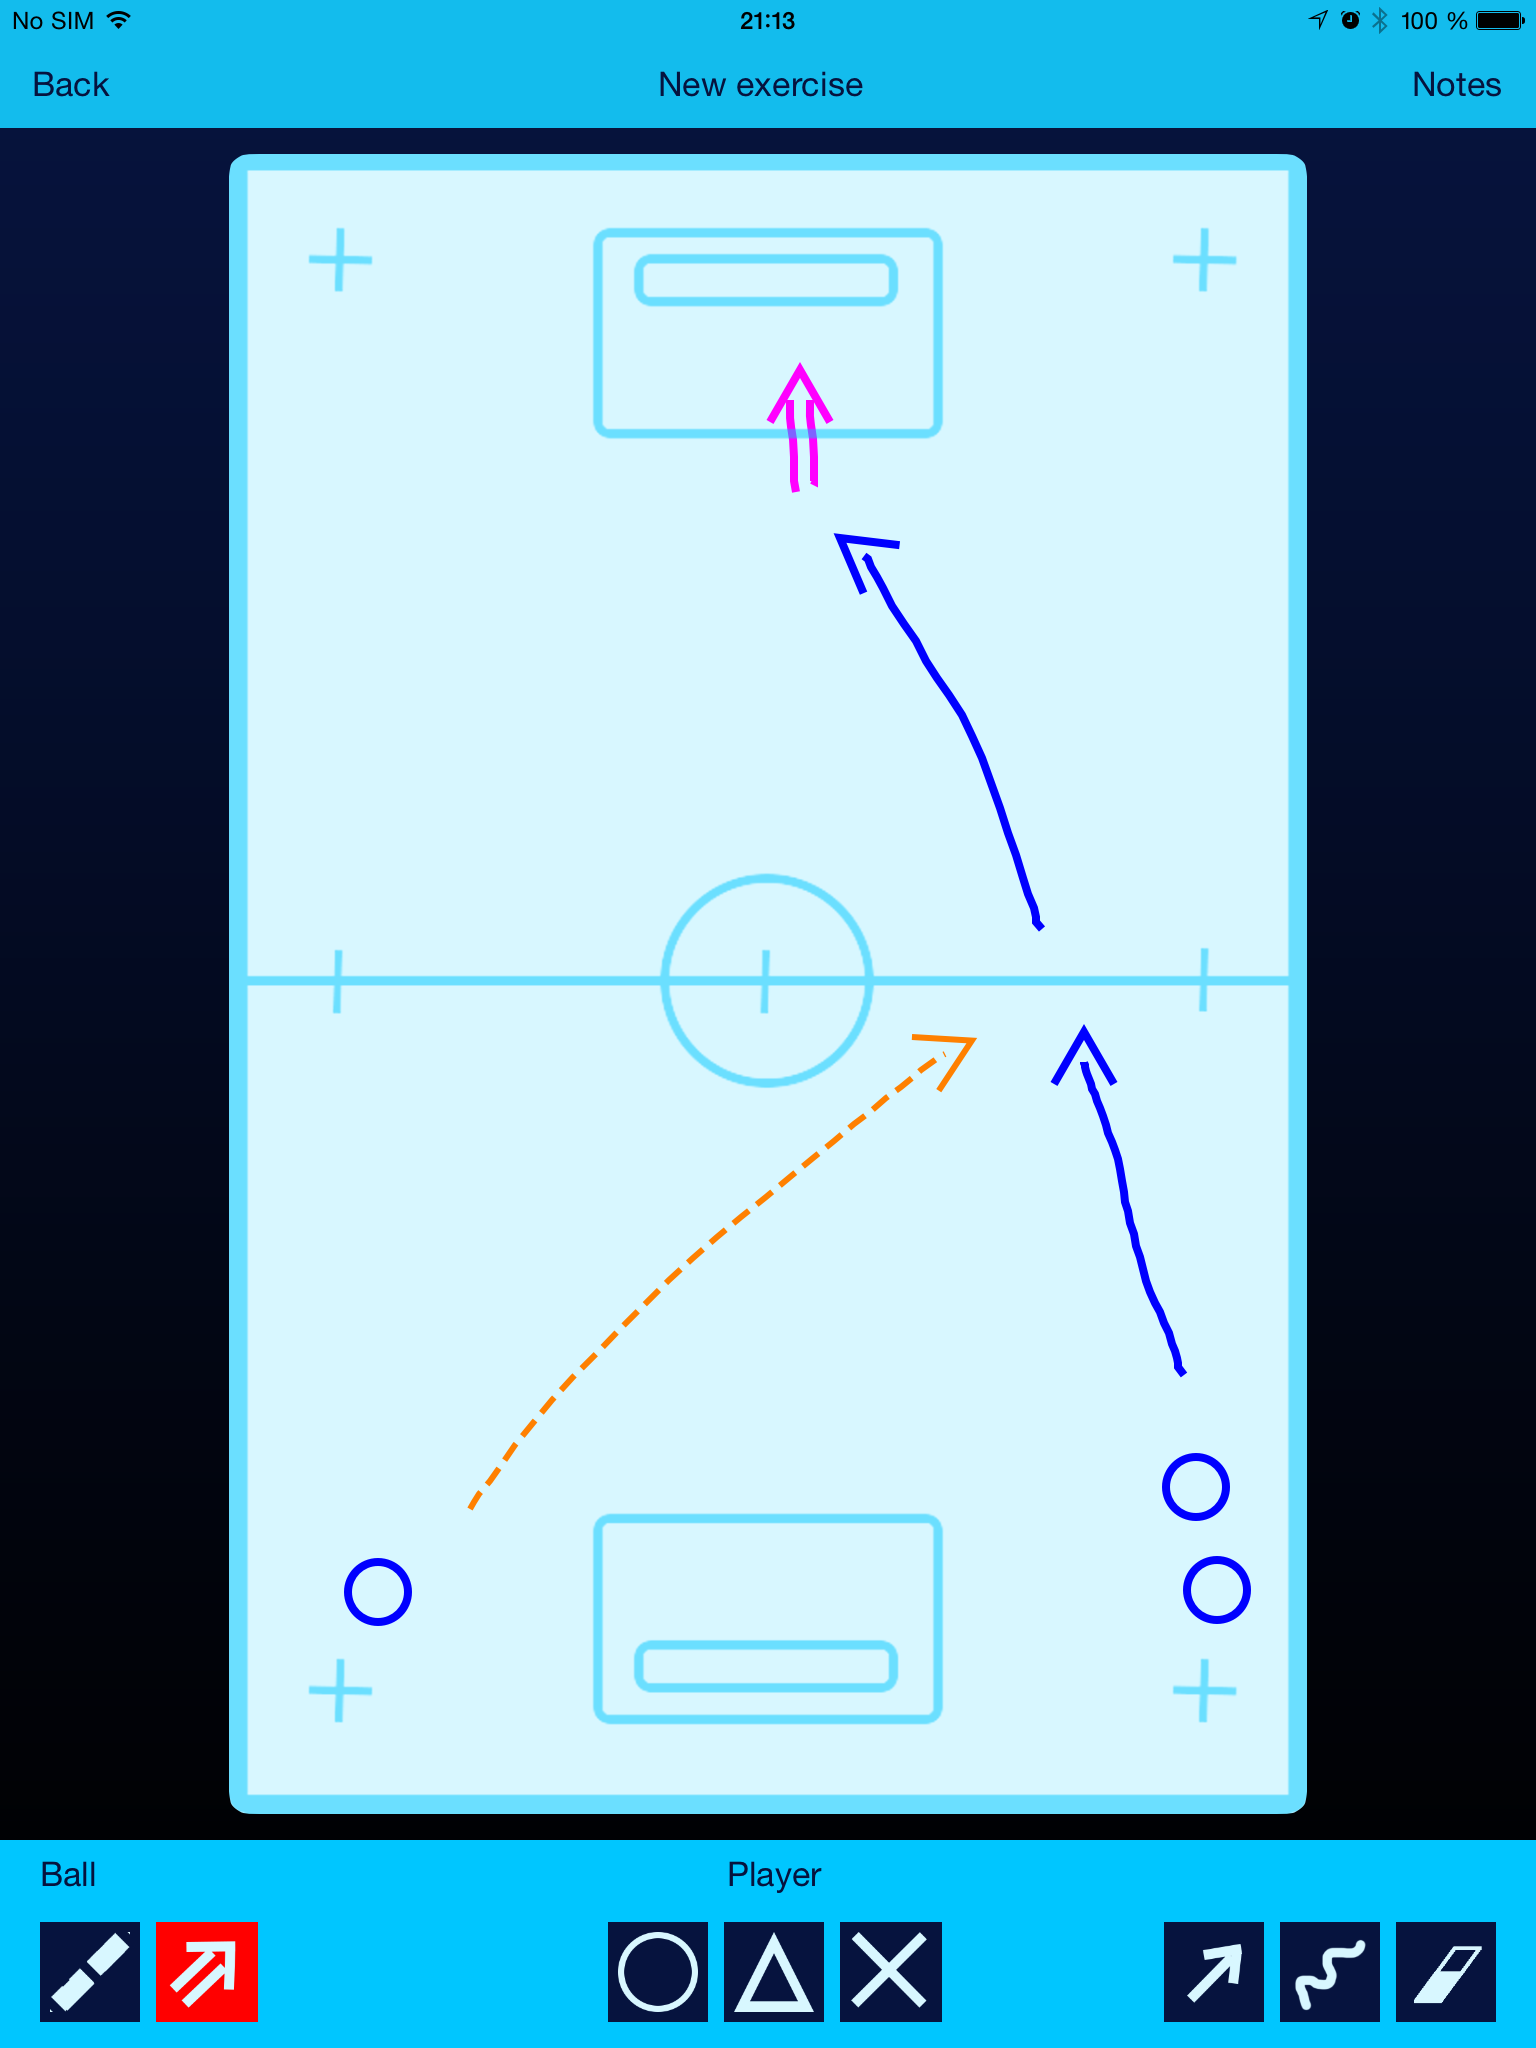
\includegraphics[width=0.4\textwidth]{img/IMG_0276}}

    \label{pic:prototype_ui}
  \end{figure}
\end{frame}

\section{Testování}

\begin{frame}
  \frametitle{Testování}
  \begin{itemize}
    \item unit testy
    \item testy uživatelského rozhraní
    \item akceptační testy
  \end{itemize}
\end{frame}

\section{Závěr}

\begin{frame}
  \frametitle{Obsah}
  \tableofcontents[currentsection]
\end{frame}

\begin{frame}
  \frametitle{Závěr}

  \begin{itemize}
    \item Implementována aplikace pro zlepšení vedení florbalových tréninků (ve fázi funkčního prototypu).
    \item Aplikace respektuje požadavky dotázaných florbalových trenérů.
    \item Analýza byla soustředěna především na podobné aplikace a požadavky budoucích uživatelů.
    \item Akceptační testy byly doplněny také o testy uživatelského rozhraní a unit testy.
  \end{itemize}
\end{frame}

\section{Otázky oponenta}

\begin{frame}
  \frametitle{Jakým způsobem a s jakými konkrétními výsledky byly provedeny akceptační testy?}

  Způsoby:

  \begin{enumerate}
    \item Vývojář podle připraveného scénáře
    \item Automatizace podle připraveného scénáře
    \item Budoucí uživatel bez připraveného scénáře
  \end{enumerate}

  Výsledky:

  \begin{itemize}
    \item U prvních dvou způsobů bylo výstupem, zda test dosáhl očekávaného výsledku.
    \item Třetí způsob byl kombinací akceptačního testu s testem uživatelského rozhraní a výstupem byl i komentář uživatele jak obtížné bylo se k očekávanému cíli dostat.
  \end{itemize}

\end{frame}
\begin{frame}
  \frametitle{Bylo řešení konzultováno s budoucími uživateli i v průběhu analýzy, návrhu a/nebo implementace?}

  \begin{itemize}
    \item Doplnění funkcí, popř. tipů na fuknce do aplikace během analýzy.
    \item Wireframy byly během návrhu upraveny podle připomínek uživatelů.
    \item Byla poskytnuta zpětná vazba vybraných trenérů během implementace.
  \end{itemize}
\end{frame}

\end{document}
